%===============================================================================
% $Id: ifacconf.tex 19 2011-10-27 09:32:13Z jpuente $  
% Template for IFAC meeting papers
% Copyright (c) 2007-2008 International Federation of Automatic Control
%===============================================================================
\documentclass{ifacconf}

\usepackage{graphicx}      % include this line if your document contains figures
\usepackage{natbib}        % required for bibliography
\usepackage{hyperref}
\usepackage{amsmath,amssymb}

% real and imaginary symbols
\renewcommand{\Re}{\operatorname{\mathbb{R}e}}
\renewcommand{\Im}{\operatorname{\mathbb{I}m}}
%===============================================================================
\begin{document}
\begin{frontmatter}

\title{Force-Limited Control of Wave Energy Converters using a Describing Function Linearization\thanksref{footnoteinfo}} 
% Title, preferably not more than 10 words.

\thanks[footnoteinfo]{This material is based upon work supported by the National Science Foundation Graduate Research Fellowship under Grant No. DGE–2139899.}

\author[First]{Rebecca McCabe} 
\author[Second]{Maha N. Haji} 

\address*{Sibley School of Mechanical and Aerospace Engineering, Cornell University, 
   Ithaca, NY 14853 USA }
   \address[First]{e-mail: rgm222@cornell.edu}
   \address[Second]{e-mail: maha@cornell.edu}

\begin{abstract}                % Abstract of not more than 250 words.
Actuator saturation is a common nonlinearity in physical systems. In wave energy conversion, force saturation can be a convenient way to limit the size and cost of the generator and the mechanical loading on the drivetrain with minimal impact on energy generation. However, such nonlinear dynamics typically demand time-domain simulation rather than frequency-domain analysis, which increases computational cost and diminishes designer intuition. This paper proposes the use of describing functions to accurately linearize the force saturation dynamics and stay in the frequency domain. It explores the impact of the force limit on electrical power production of a generic single-body wave energy converter under energy-maximizing reactive control. A sweep of nondimensional coefficients is carried out to visualize the effect of the maximum force value on devices with different hydrodynamics and powertrain dynamics. Sensitivity results are discussed in the context of sizing drivetrain components such as the generator. The describing function method is over 200 times faster than a time-domain simulation and X times faster than a spectral-domain simulation, showing promise as a technique to enable future studies such as large-scale design optimization and control co-design.
\end{abstract}

\begin{keyword}
Constrained control, control of renewable energy resources, systems with saturation, nonlinear and optimal marine system control, sensors and actuators.
\end{keyword}

\end{frontmatter}
%===============================================================================

\section{Introduction}
Final page limit is 6, initial submissions can be 8 pages

\subsection{Motivation}
Motivation for caring about force saturation: the maximum force in the powertrain drives generator sizing and drivetrain loading, and therefore cost. We want to trade off reduced power for reduced force.

Motivation for wanting analysis that is analytical and linear: intuition, use the abundance of linear system analysis tools, computational efficiency, ability to couple with other subsystem models to do CCD and MDO

\subsection{Literature Review}
NUMERICAL (Most of the work in this space is numerical constrained optimal control, typically using either MPC or spectral/pseudo-spectral methods.)
- WecOptTool CCD paper \cite{strofer_control_2023}
- Ringwood paper from IFAC last year that's very similar to mine and includes an economic model and the effect on LCOE \cite{pena-sanchez_control_2022}
- Sichani sweeps force constraints numerically and shows that optimal damping gets higher as constraint gets lower, and optimal stiffness changes slightly \cite{sichani_constrained_2014}
- Babarit 2023 PTO capping: effect of 3 different force caps and 3 different power caps on the energy spectrum, with energy calculated from real sea data in 4 different ways. The focus is not on the energy but on the accuracy of the energy prediction in different calculation methods. \cite{de_la_torre-castro_combined_2023}
- Many people doing MPC with constraints
- Tedeschi 2011 power saturation with simulink \cite{tedeschi_effect_2011}
- NREL 2017 PS with load capping \cite{tom_pseudo-spectral_2017}
- Dan Herber 2014 \cite{herber_wave_2014}

ANALYTICAL (A minority of papers tackle the problem analytically
- Flower and Knott 1979 describing function for nonlinear pto damping intended to incorporate friction. This is the only relevant paper I could find in the WEC space that uses describing functions. \cite{flower_describing-function_1980}
- Giorgio's paper with the geometric tool for simultaneous force and position constraints. Uses the spectral method (Galerkin's method) but needs to approximate constraints with their 2-norm (effectively constraining the RMS rather than the peak). Accounts for interaction of both force and position constraint at once. \cite{bacelli_geometric_2013}
- Zou and Bacelli 2017 analytical solution showed that bang-singular arc-bang controller is optimal (saturate the unsaturated solution) using the Pontryagin maximum principle \cite{zou_optimal_2017}
- Abdulakir 2024 extend the above work to arrays \cite{abdulkadir_optimal_2024}
- Both of the two above papers give the analytical expression for the optimal control force but do not (as far as I could see? double check this) show the effect on power because you still need a time domain simulation of that optimal force to see what it does.

STILL NEED TO CHECK
- Giorgio's paper that implements constraints for a real WEC (+thesis?)
- Ringwood follow on paper for pneumatic valve

non WEC:
- 2021 Japanese paper uses describing functions to model velocity saturation and torque saturation on a two-motor impedance-controlled system for a robotics application, and experimentally validates their results \cite{fukui_impedance_2021}

\subsection{Paper Contribution and Outline}
Wave energy converters are designed to resonate with incoming waves, and maximum power transfer requires impedance matching of the powertrain, controller, and hydrodynamic body. Actuator limitations can make this perfect impedance matching impossible. In this sense, force saturation can be seen as an impedance mismatch. Therefore, before analyzing the nonlinear dynamics of saturation, it is first informative to examine the properties of an impedance-mismatched linear system. This is outlined and visualized in section~\ref{sec:linear}, starting for a general system and then moving to an oscillating-body wave energy converter specifically. In section~\ref{sec:nonlinear}, the describing function is introduced to handle the saturation nonlinearity, providing an intuitive linear approximation. Sensitivity results are provided in section~\ref{sec:sensitivities}, focusing on implications in powertrain sizing.

\section{Peak Limiting in the Linear Case}\label{sec:linear}
\subsection{General Impedance-Matched System}
The analysis starts with a generic linear system modeled as a Thévenin equivalent circuit with AC voltage source $V_{th}$ and complex source impedance $Z_{th}$, shown in Fig.~\ref{fig:circuit}. The load impedance $Z_L$ is to be selected, with the conflicting goals of maximizing average power transfer $\overline{P}_L$ and minimizing the peak amplitude of load current $|I_L|$ or voltage $|V_L|$. Maximum power transfer occurs at $Z_L = Z_{th}^*$ where $*$ indicates the complex conjugate. The load average power, peak voltage, and peak current at this matched point, denoted $\overline{P}_L^m, |V_L^m|,$ and $|I_L^m|$ respectively, are found as
\begin{equation}
    \overline{P}_L^m = \frac{|V_{th}|^2}{8 \Re(Z_{th})}, 
    |V_L^m| = \frac{|V_{th}| |Z_{th}|} {2 \Re(Z_{th})}, 
    |I_L^m| = \frac{|V_{th}|}{2 \Re(Z_{th})}
\end{equation}

\begin{figure}
\begin{center}
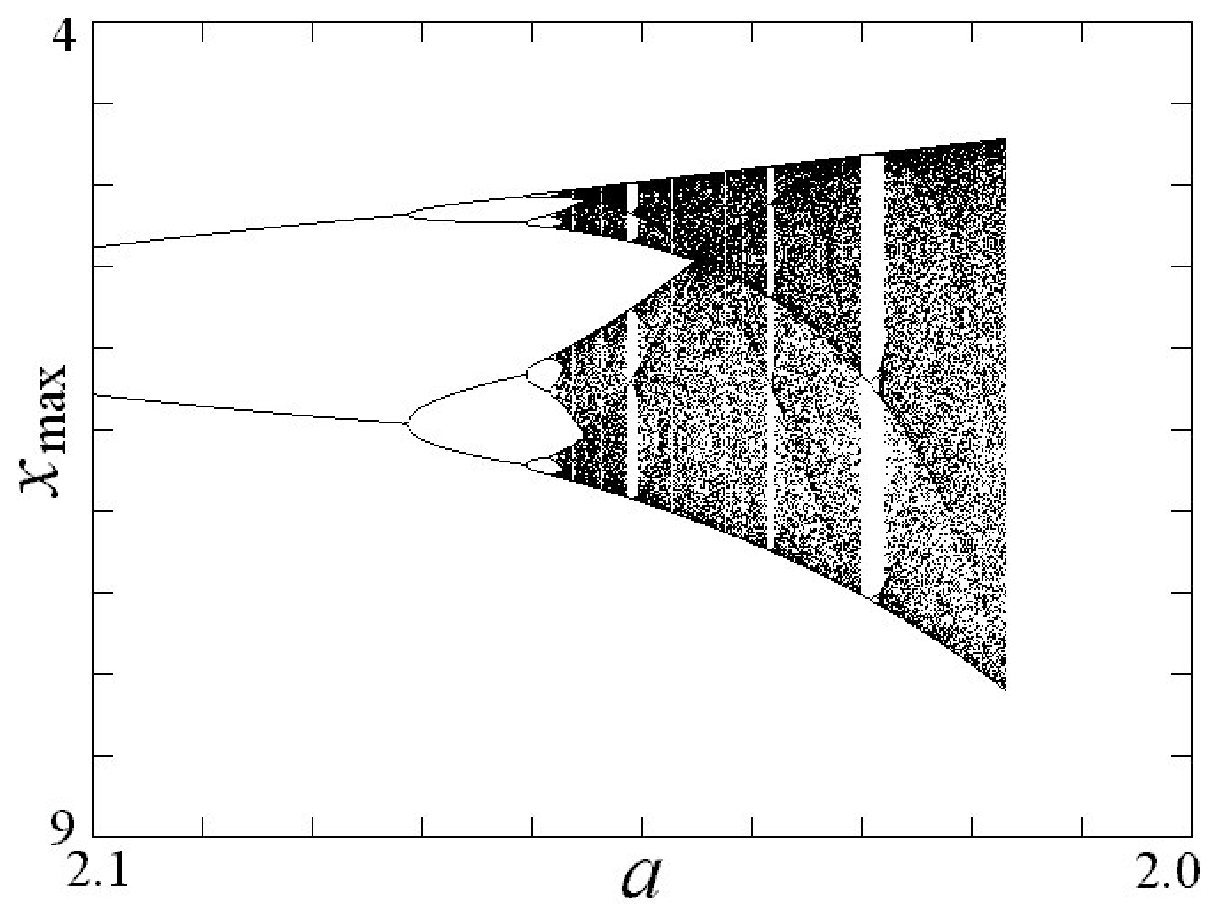
\includegraphics[width=8.4cm]{bifurcation}    % The printed column width is 8.4 cm.
\caption{Thévenin equivalent circuit for linear system} 
\label{fig:circuit}
\end{center}
\end{figure}

To consider all possibilities of the unmatched case, we set $Z_L = z Z_{th}^*$ for arbitrary complex number $z$. The space of $z$ can be visualized using a Smith chart, where $\Re(z)$ is on a curved horizontal axis and $\Im(z)$ is on a curved vertical axis. The axes are curved such that the chart can be simultaneously read as a standard polar plot of the complex reflection coefficient $\Gamma$, which is a transformation of $z$ defined as $\Gamma = \frac{z-1}{z+1}$. The impedance-matched case of $z=1$, $\Gamma = 0$ is found at the center of the plot, the minimum voltage $z=0$, $\Gamma = -1$ on the left, and the minimum current $z \rightarrow \infty$, $\Gamma = 1$ on the right.

If the impedance match is imperfect, the average power, peak voltage, and peak current can be found as fractions of their matched counterparts using standard circuit techniques:
\begin{equation}\label{eq:ratios}
\begin{aligned}
     \frac{\overline{P}_L}{\overline{P}_L^m} &= 1 - |\Gamma|^2\\
     \frac{|V_L|}{|V_L^m|} &= \sqrt{\frac{|\Gamma|^2 + 2 \Re(\Gamma) + 1}{\theta^2 |\Gamma|^2 + 2 \theta \Im(\Gamma) + 1} } \\
     \frac{|I_L|}{|I_L^m|} &= \sqrt{\frac{|\Gamma|^2 - 2 \Re(\Gamma) + 1}{\theta^2 |\Gamma|^2 + 2 \theta \Im(\Gamma) + 1} }\\
\end{aligned}
\end{equation}
The voltage and current relationships in (\ref{eq:ratios}) depend not only on $\Gamma$ but also on the phase of $Z_{th}$ via the parameter $\theta = \frac{\Im(Z_{th})}{\Re(Z_{th})}$. These relationships are visualized on the Smith charts in Fig.~\ref{fig:power-smith}.

\begin{figure}
\begin{center}
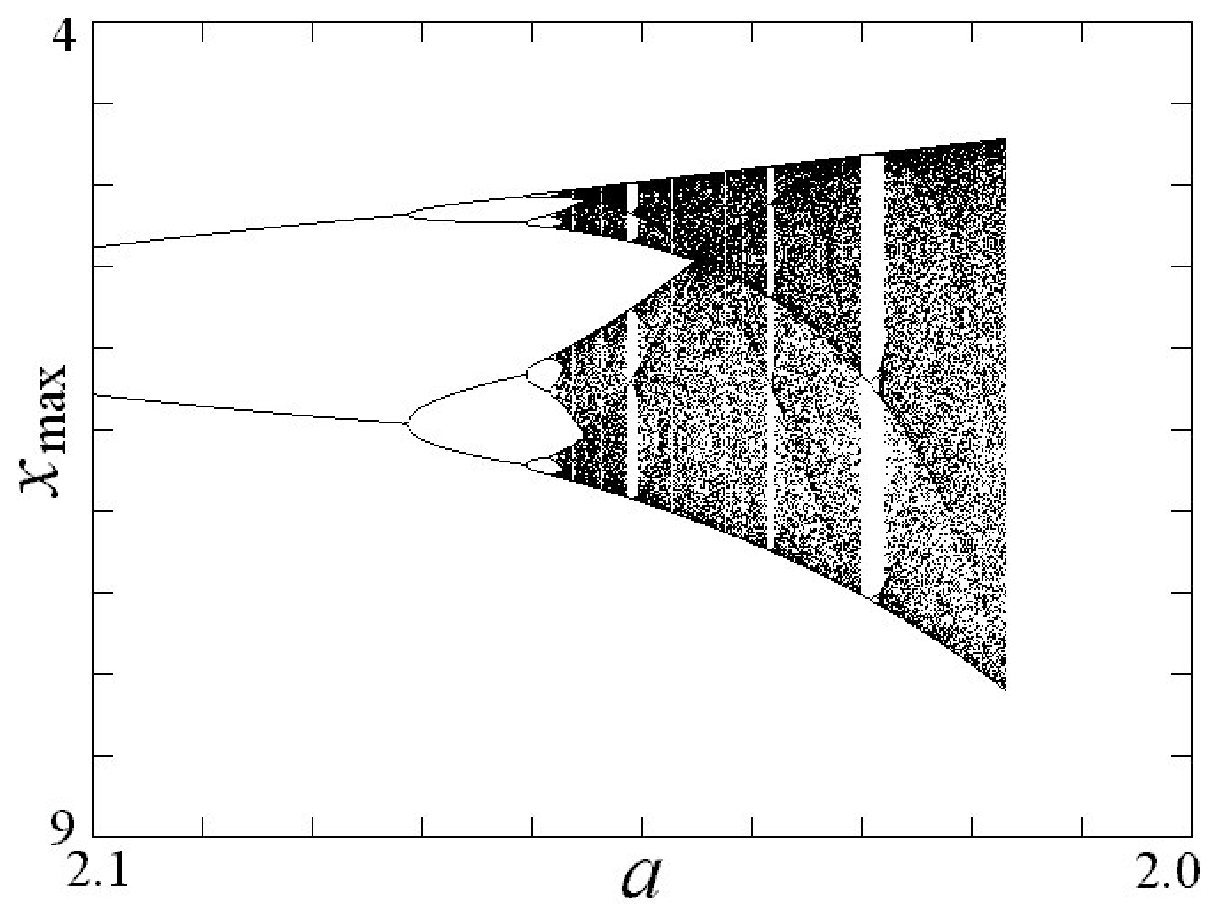
\includegraphics[width=8.4cm]{bifurcation}    % The printed column width is 8.4 cm.
\caption{Smith charts representing the average power, peak voltage, and peak current at the load for any $z=\frac{Z_L}{Z_{th}}$.} 
\label{fig:power-smith}
\end{center}
\end{figure}

On these plots, shaded in grey are points where the respective values exceed 1. These points are undesirable because they absorb less power than the matched case while having higher peaks. The pareto-optimal contours (highest $\frac{|V_L|}{|V_L^m|}$ and $\frac{|I_L|}{|I_L^m|}$ for a given $\frac{\overline{P}_L}{\overline{P}_L^m}$) are traced out with dashed lines. This optimal tradeoff $(\cdot)^\textrm{opt}$ can be found analytically by setting the partial derivative of $\frac{|V_L|}{|V_L^m|}$ and $\frac{|I_L|}{|I_L^m|}$ with respect to $\angle~\Gamma$ equal to zero:
\begin{equation}\label{eq:optimal-vi}
\begin{aligned}
    \frac{|V_L|}{|V_L^m|}^\textrm{opt} &= 2 \tan^{-1}{ \frac{\theta^2 |\Gamma|^2 - \sqrt{(\theta^2 + 1)(\theta^2 |\Gamma|^4 + 1)} + 1}{\theta (1 - |\Gamma|)^2}} \\
    \frac{|I_L|}{|I_L^m|}^\textrm{opt} &= -2 \tan^{-1}{ \frac{\theta^2 |\Gamma|^2 - \sqrt{(\theta^2 + 1)(\theta^2 |\Gamma|^4 + 1)} + 1}{\theta (1 + |\Gamma|)^2}}
\end{aligned}
\end{equation}

These pareto-optimal contours are aggregated in Fig.~\ref{fig:pareto} to show the tradeoff between power and voltage/current. Interestingly, as $|\theta|$ grows (i.e., as $Z_{th}$ becomes less resistive and more reactive), there is less of a power penalty for a given voltage or current reduction. In other words, the power in the pure resistive $Z_{th}$ case is the most sensitive to voltage and current reductions.

Note that when following the optimal contours, it may require a $z$ with nonzero imaginary part, i.e. a $Z_L$ that is more or less reactive than the impedance-matched case, rather than merely scaled up or down. Furthermore, because the optimal voltage reduction path requires decreasing the impedance and the optimal current reduction path requires increasing the impedance, it is not possible to follow both paths simultaneously. For sufficiently high values of $\theta$, it is possible to reduce both current and voltage simultaneously (i.e. avoid the shaded region of both smith charts), although for $\theta=0$ a decrease in voltage is always associated with an increase in current. This tradeoff is explored further in Fig.~\ref{fig:pareto}.

These plots reveal the effect of an impedance mismatch on power, current, and voltage, and can be used to choose an appropriate load impedance based on the relative importance of power generation and peak limiting. 
% Considering a weighted linear objective function $J$ 

% \begin{equation}
%     J = a~ \frac{\overline{P}_L}{\overline{P}_L^m} - b~ \frac{|V_L|}{|V_L^m|} - (1 - a - b)~ \frac{|I_L|}{|I_L^m|}
% \end{equation}
% for $0 \leq a, b \leq 1$, we can substitute (\ref{eq:ratios}) and differentiate to derive the $\Gamma$ which maximizes $J$:

% \begin{equation}
%     \Gamma^\textrm{opt} = f(a, b, \theta)
% \end{equation}
% This tradeoff is shown

% Note that substituting $a=1, b=0$ recovers the optimal current condition and $a=1, b=1$ the optimal voltage condition from (\ref{eq:optimal-vi}).

\subsection{Wave Energy Converters}
Insert block diagram here
Derive $Z_{th}$ and $V_{th}$ as a function of $\zeta_u$ and $\omega_u^*$, and derive $\zeta_u$ and $\omega_u^*$ as a function of hydro params and drivetrain params 


\section{Saturation Nonlinearities and Describing Functions}\label{sec:nonlinear}

\subsection{Theory}
The control law used in this section is $F_{p,sat}(t) = F_{max}\textrm{sat}(F_p(t)/F_{max})$. If we assume the powertrain force profile is a saturated sinusoid (which is very close but not exact because harmonics in $x$ and $\dot{x}$ will make the unsaturated signal already contain content other than the fundamental), we can decompose this nonlinear force signal into the sum of the fundamental and higher harmonics: 
\begin{equation}
    F_{p,sat}(t) \approx \sum_i |F_{p,sat,i}| \sin(i \omega t + \psi)
\end{equation} where $\psi$ is the same phase as the unsaturated $F_p$ had. The amplitude of the $i$th powertrain force harmonic $|F_{p,sat,i}|$ is equal to $f_{sat,i} |F_p|$, where $f_{sat,i}$ is a saturation factor compared to the unsaturated powertrain force amplitude $|F_p|$.
\begin{equation}\label{f-sat-i-defn}
    f_{sat,i} = \frac{|F_{p,sat,i}|}{|F_p|} = \frac{|F_{p,sat,i}|}{\sqrt{(B_p\omega)^2+K_p^2}~|X|}
\end{equation}

To find $f_{sat,i}$, we can apply the describing function technique, leveraging Fourier analysis of a saturated sin wave to get an equivalent linear transfer function for the nonlinear system:
\begin{equation}\label{f-sat-desc-fcn}
    f_{sat,i} =
\begin{cases}
1 & \quad |F_p| \leq F_{max} \And i = 1\\
0 & \quad |F_p| \leq F_{max} \And i \neq 1 \\
\frac{2}{\pi} \left(\frac{F_{max}}{|F_p|}\sqrt{1 - \left(\frac{F_{max}}{|F_p|}\right)^2} + \theta \right) & \quad |F_p| > F_{max} \And i = 1 \\ 
0 & \quad |F_p| > F_{max} \And i = 2,4,6,... \\
\frac{4}{\pi} \frac{1}{i (i^2 - 1)} \left( i \sqrt{1 - (\frac{F_{max}}{|F_p|})^2}\sin(\theta) - \frac{F_{max}}{|F_p|}\cos(\theta) \right) & \quad |F_p| > F_{max} \And i = 3,5,7,...
\end{cases}
\end{equation}
where $\theta = i \sin^{-1}\frac{F_{max}}{|F_p|} $

This is shown in Figure \ref{fig:desc-fcn} for the first 7 harmonics. As the amount of saturation increases, the fundamental amplitude decreases, and the higher harmonics become more prominent. The limit for large $\frac{F_{max}}{|F_p|}$ is a square wave.

\begin{figure}
    \centering
    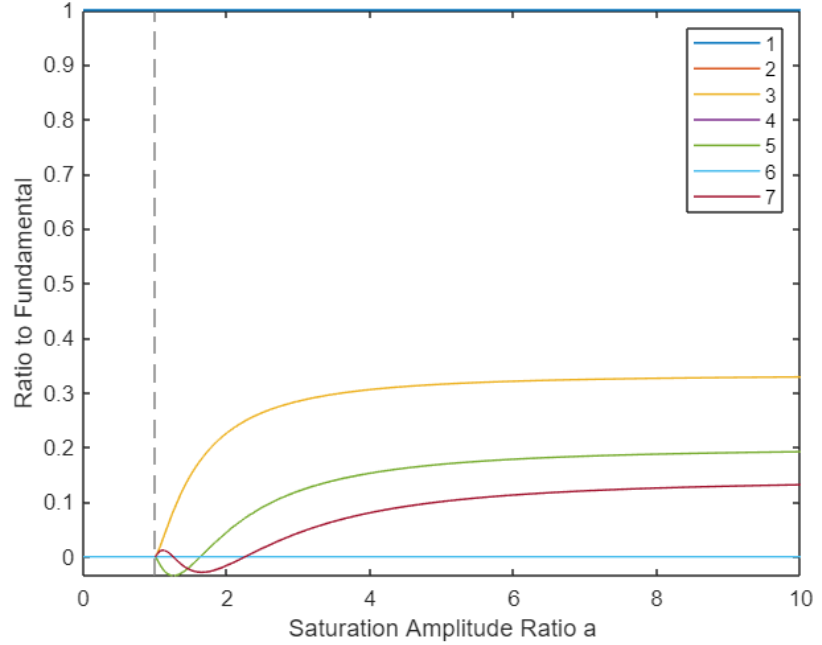
\includegraphics[width=8.4cm]{ifacconf_latex/saturation_harmonics.png}
    \caption{Enter Caption}
    \label{fig:desc-fcn}
\end{figure}

So we see that the force applied by the saturated controller can be approximated by a sum of scaled-down responses to unsaturated controllers:
\begin{equation}\label{m-sat-intro}
\begin{aligned}
    \frac{|F_{p,sat,i}|}{|X_{sat,i}|} &\approx m_{sat,i} \frac{|F_{p,i}|}{|X_i|} = m_{sat,i} \sqrt{ (B_p i \omega)^2 + K_p^2} \\
    F_{p,sat}(t) &\approx \sum_i m_{sat,i} \sqrt{ (B_p i \omega)^2 + K_p^2} ~|X_{sat,i}| \sin(i \omega t + \psi) \\
    &\approx \sum_i m_{sat,i} (B_p \dot{x}_{sat,i} + K_p x_{sat,i} )
\end{aligned}
\end{equation}
where $m_{sat,i}$ is a gain multiplier calculated as a function of $f_{sat,i}$ and the dynamics. The same multiplier is applied to the damping $B_p$ and the stiffness $K_p$ because this preserves the phase of the $F_p$ waveform, and saturating a sin does not change its phase.

Applied to the full system dynamic response:
\begin{equation}
    \sum_i \left[ m \ddot{x}_{sat,i} + (B_h+m_{sat,i}B_p) \dot{x}_{sat,i} + (K_h + m_{sat,i}K_p) x_{sat,i} \right] \approx F_h \sin(\omega t)
\end{equation}
Now we have a quasi-linear system, where the response is the sum of linear responses at different frequencies.

\subsubsection{Only considering the fundamental frequency}
It is a reasonable approximation to only consider $f_{sat,1}$ the fundamental force harmonic, because the system is essentially a second order low pass filter, so the higher harmonics are attenuated and contain little energy. In this section, we make this additional approximation and use $m_{sat}$ and $f_{sat}$ to refer to $m_{sat,1}$ and $f_{sat,1}$ respectively.

The new dynamics are fully linear:
\begin{equation}
    m \ddot{x}_{sat} + (B_h+m_{sat}B_p) \dot{x}_{sat} + (K_h + m_{sat}K_p) x_{sat} \approx F_h \sin(\omega t)
\end{equation}

The gain multiplier $m_{sat}$ must be calculated from $f_{sat}$ such that the resulting saturated powertrain force is a factor $f_{sat}$ times the unsaturated powertrain force. From \eqref{f-sat-i-defn} and \eqref{m-sat-intro}, we have:
\begin{equation} \label{eq:force-sat}
    m_{sat} = f_{sat} \frac{|X|} {|X_{sat}|}
\end{equation} 
Substituting \eqref{x-magnitude} for both the saturated and unsaturated powertrain coefficients into \eqref{eq:force-sat} reveals that $m_{sat}$ is the solution to a quadratic equation $a_q m_{sat}^2 + b_q m_{sat} + c_q = 0$, where the quadratic coefficients can be expressed as:
\begin{equation}\label{abc-matrix}
    \begin{bmatrix}
        a_q \\ b_q \\ c_q
    \end{bmatrix}
    = 
    \begingroup % keep the row spacing change local
    \setlength\arraycolsep{2pt}
    \begin{bmatrix*}[r] -4 & 0 & \frac{1}{f_{sat}^2} & 0 & -1\\
    8 & -8 & 0 & 2 & 2\\ -4 & 8 & -1 & -2 & -1 \end{bmatrix*}
    \endgroup
    \begin{bmatrix*}[l] 
    ~~~~{r_{k}}^2\left(\zeta^2\,\omega^{*2} \right)  \\
    r_{b}~\,{r_{k}}^2  \left(\zeta^2\,\omega^{*2} \right) \\
    {r_{b}}^2{r_{k}}^2 \left( \omega^{*4}+ 4\zeta^2\omega^{*2} - 2\,\omega^{*2} + 1 \right) \\
    {r_{b}}^2\,r_{k}\,\left(\omega^{*2} \, -1\right) \\
    {r_{b}}^2 ~~~~\left(1 \right)  
    \end{bmatrix*}
\end{equation}

Here we have introduced nondimensional ratios $r_k$ and $r_b$ to represent the relative magnitude of the total stiffness and damping to the powertrain stiffness and damping, $\omega^*$ for the ratio of the wave frequency to the system natural frequency, and $\zeta$ for the system damping ratio. These substitutions make \eqref{abc-matrix} fully nondimensional, which aids intuition in understanding how $m_{sat}$ changes based on the sea state.

\begin{equation}
    r_k = \frac{k}{K_p} = \frac{K_h+K_p}{K_p}
\end{equation}
\begin{equation}
    r_b = \frac{b}{B_p} = \frac{B_h+B_p}{B_p}
\end{equation}
\begin{equation}
    \omega^* = \frac{\omega}{\omega_n} = \frac{\omega}{\sqrt{k/m}}
\end{equation}
\begin{equation}
    \zeta = \frac{b}{2\sqrt{km}}
\end{equation}
Todo: express \eqref{abc-matrix} as a function of $r_b$, $\omega^*$, $\zeta_u$, and $\omega_u^*$ instead of $r_b$, $\omega^*$, $\zeta$, and $r_k$ to be consistent with the nondimensionalization in the previous section.

The no saturation case ($f_{sat} = 1$) for \eqref{abc-matrix} yields $m_{sat}=1$. This confirms the expected behavior that when no force reduction is required, the powertrain coefficients can remain unchanged.

As derived in a previous section, optimal-power reactive control requires $r_b = 2$ and $\omega^* = 1$. Substituting these into \eqref{abc-matrix} and solving the quadratic results in the following expression for $m_{sat}$:
\begin{equation}\label{eq:m-sat}
    m_{sat} = \frac{-f_{sat}\,\left(f_{sat}\,{(r_k \zeta)}^2-f_{sat}+2\,\left|r_k \zeta\right|\,\sqrt{-f_{sat}^2+{(r_k \zeta)}^2+1}\right)}{f_{sat}^2\,{(r_k \zeta)}^2+f_{sat}^2-4\,{(r_k \zeta)}^2}
\end{equation}
Here the relationship between $m_{sat}$ and $f_{sat}$ depends on the product $|r_k \zeta|$, which in the optimal-power reactive control case can be expressed in terms of hydrodynamic coefficients:
\begin{equation}
    |r_k \zeta| = \left| \frac{\omega^*_u/\omega^*}{(\omega^*_u/\omega^*)^2 - 1} \frac{r_b}{r_b - 1} \zeta_u \right| = \left|\frac{\omega B_h} {m \omega^2 - K_h}\right|.
\end{equation}

We try plugging in real values for $B_h(\omega)$ and $m(\omega)$ from hydrodynamic simulations of a hollow cylinder geometry. The resulting $|r_k \zeta|$ is less than one for most frequencies, but rises toward infinity around the device's natural resonant frequency under no control input, $\omega_{n,u}$. Figure \ref{fig:r-k-zeta-vs-freq} shows the relationship for the nominal and optimal designs. 

\begin{figure}[h]
    \centering
    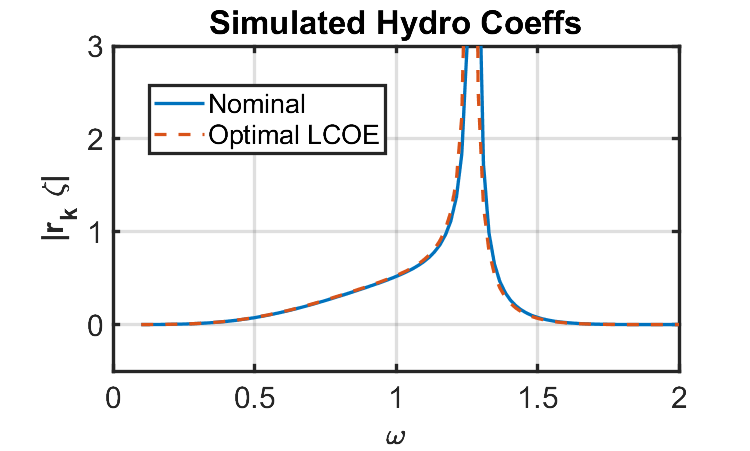
\includegraphics[width=\linewidth]{rk_zeta_vs_omega.png}
    \caption{Caption}
    \label{fig:r-k-zeta-vs-freq}
\end{figure}

After plugging in $X_{sat}(f_{sat},m_{sat})$ into \eqref{power-any-control}, we see that energy generation scales with $e = f_{sat}^2/m_{sat}$. This can provide insight on how force saturation affects energy generation at various frequencies and hydrodynamic designs.
\begin{figure}[!hbt]
    \centering
    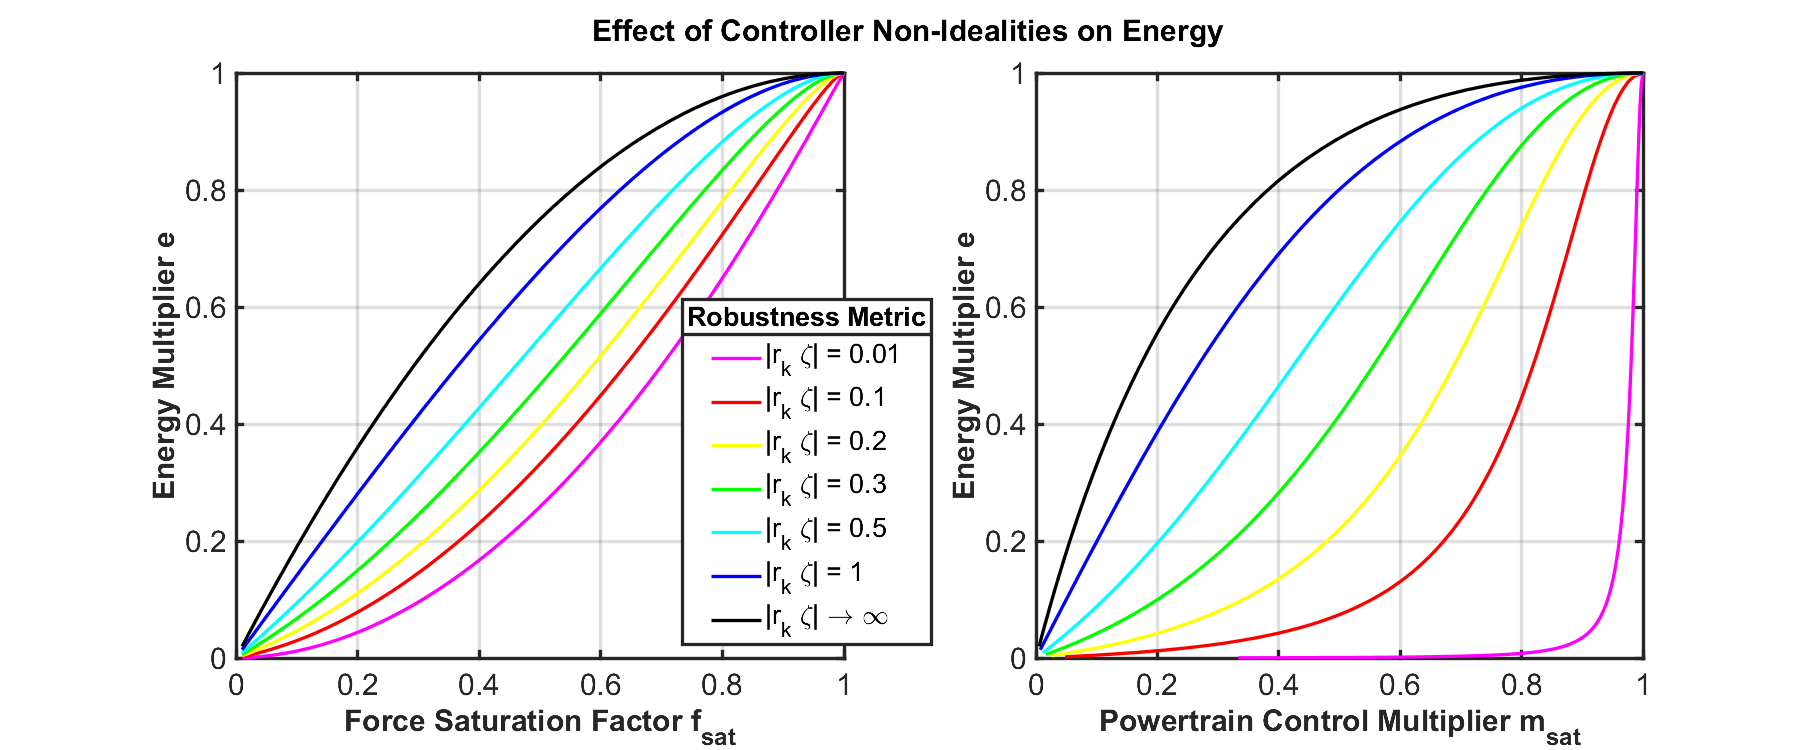
\includegraphics[width=\linewidth]{saturation-rk-zeta-2.png}
    \caption{Caption}
    \label{fig:my_label}
\end{figure}

$|r_k \zeta|$ can be thought of as a robustness metric, with higher $|r_k \zeta|$ meaning that the hydrodynamic design is more robust to controller non-idealities. The plot on the left shows that for large $|r_k \zeta|$, a given force saturation requirement will have less of an effect on the energy production. With these same relationships, we can also interpret robustness more broadly, not only describing the response to force saturation but also to differences between the intended control gains and the actual ones. For example, the right plot shows that for $|r_k \zeta| = 0.01$, if the actual control gains are 10\% lower than intended ($m_{sat} = 0.9$), then only one twentieth of the expected power is generated ($e = 0.05$).

Design takeaway: force saturation will have the least impact on energy generation when the excitation frequency equals the uncontrolled natural frequency (pure hydrodynamic response) $\omega_{n,u}$. For typical hydrodynamic coefficients, excitation frequencies higher than $\omega_{n,u}$ abruptly result in less energy, and excitation frequencies lower than $\omega_{n,u}$ more gradually result in less energy. This suggests that for force-limited systems, it may make sense to design $\omega_{n,u}$ to be higher than it would be in an unsaturated system, to avoid the steep dropoff in energy at the ocean excitation frequencies. This is very promising because $\omega_{n,u} = \sqrt{\frac{K_h}{m}}$, and lowering the mass would achieve the desired increase in $\omega_{n,u}$ while also decreasing structural costs.

\subsubsection{Including higher harmonics}
Todo. Use the expression for $f_{sat,i}$ for i=3,5,7... in \eqref{f-sat-desc-fcn} to approximate the energy in the higher harmonics. I think the inclusion of higher frequencies of the describing function is the so-called ``Higher order sinusoidal input describing functions" method (Nuji, Bosgra, and Steinbuch 2006).

\subsection{Limitations}
The main limitation of the describing function is that it only applies to regular waves. The saturated sinusoid shape of the force waveform relies on a sinusoidal wave. Real waves come from a broadband spectrum and are irregular. It remains to be tested how accurate the results are for irregular waves. Even for regular waves, describing functions still are approximations that rely on the low pass filter behavior of the WEC. For WECs that are broadband, such as small WECs, this assumption may be poor. Future work includes a full error analysis of the describing functions compared to a fully nonlinear simulation.

\section{Sensitivities}\label{sec:sensitivities}
\subsection{Nondimensional Results}
\subsection{Dimensional Generator Sizing Implications}

%% There are a number of predefined theorem-like environments in
%% ifacconf.cls:
%%
%% \begin{thm} ... \end{thm}            % Theorem
%% \begin{lem} ... \end{lem}            % Lemma
%% \begin{claim} ... \end{claim}        % Claim
%% \begin{conj} ... \end{conj}          % Conjecture
%% \begin{cor} ... \end{cor}            % Corollary
%% \begin{fact} ... \end{fact}          % Fact
%% \begin{hypo} ... \end{hypo}          % Hypothesis
%% \begin{prop} ... \end{prop}          % Proposition
%% \begin{crit} ... \end{crit}          % Criterion
%% \begin{pf} ... \end{pf}              % Proof


\section{Helpful Hints}
\subsection{Tables}
Tables must be centered and have a caption above them, numbered with
Arabic numerals. See table~\ref{tb:margins} for an example.

\begin{table}[hb]
\begin{center}
\caption{Margin settings}\label{tb:margins}
\begin{tabular}{cccc}
Page & Top & Bottom & Left/Right \\\hline
First & 3.5 & 2.5 & 1.5 \\
Rest & 2.5 & 2.5 & 1.5 \\ \hline
\end{tabular}
\end{center}
\end{table}

\subsection{Final Stage}

\subsection{Units}

Use SI as primary units. Other units may be used as secondary units
(in parentheses). This applies to papers in data storage. For example,
write ``$15\,\mathrm{Gb}/\mathrm{cm}^2$ ($100\,\mathrm{Gb}/\mathrm{in}^2$)''. 
An exception is when
English units are used as identifiers in trade, such as ``3.5 in
disk drive''. Avoid combining SI and other units, such as current in
amperes and magnetic field in oersteds. This often leads to confusion
because equations do not balance dimensionally. If you must use mixed
units, clearly state the units for each quantity in an equation.  The
SI unit for magnetic field strength $\mathbf{H}$ is $\mathrm{A}/\mathrm{m}$. However, if you wish to
use units of $\mathrm{T}$, either refer to magnetic flux density $\mathbf{B}$ or
magnetic field strength symbolized as $\mu_0\,\mathbf{H}$. Use the center dot to
separate compound units, e.g., ``$\mathrm{A} \cdot \mathrm{m}^2$''.

\subsection{Figures and Tables}

Figure axis labels are often a source of confusion. Use words rather
than symbols. As an example, write the quantity ``Magnetization'', or
``Magnetization M'', not just ``M''. Put units in parentheses. Do not
label axes only with units.  For example, write ``Magnetization
($\mathrm{A}/\mathrm{m}$)'' or ``Magnetization ($\mathrm{A} \mathrm{m}^{-1}$)'', not just
 ``$\mathrm{A}/\mathrm{m}$''. Do not
label axes with a ratio of quantities and units. For example, write
``Temperature ($\mathrm{K}$)'', not ``$\mbox{Temperature}/\mathrm{K}$''.

Multipliers can be especially confusing. Write ``Magnetization
($\mathrm{kA}/\mathrm{m}$)'' or ``Magnetization ($10^3 \mathrm{A}/\mathrm{m}$)''. Do not write
``Magnetization $(\mathrm{A}/\mathrm{m}) \times 1000$'' because the reader would not know
whether the axis label means $16000\,\mathrm{A}/\mathrm{m}$ or $0.016\,\mathrm{A}/\mathrm{m}$.

\subsection{References}

Use Harvard style references (see at the end of this document). Please note that the references at the end of this
document are in the preferred referencing style. Papers that have not
been published should be cited as ``unpublished''.  Capitalize only the
first word in a paper title, except for proper nouns and element
symbols.

\subsection{Abbreviations and Acronyms}

Define abbreviations and acronyms the first time they are used in the
text, even after they have already been defined in the
abstract. Abbreviations such as IFAC, SI, ac, and dc do not have to be
defined. Abbreviations that incorporate periods should not have
spaces: write ``C.N.R.S.'', not ``C. N. R. S.''

\subsection{Equations}

Number equations consecutively with equation numbers in parentheses
flush with the right margin, as in (\ref{eq:sample}). Punctuate equations when they are part of a sentence, as
in

\begin{equation} \label{eq:sample2}
\begin{array}{ll}
\int_0^{r_2} & F (r, \varphi ) dr d\varphi = [\sigma r_2 / (2 \mu_0 )] \\
& \cdot \int_0^{\inf} exp(-\lambda |z_j - z_i |) \lambda^{-1} J_1 (\lambda  r_2 ) J_0 (\lambda r_i ) d\lambda 
\end{array}
\end{equation}

Be sure that the symbols in your equation have been defined before the
equation appears or immediately following. Italicize symbols ($T$
might refer to temperature, but T is the unit tesla).

\subsection{Other Recommendations}

Hyphenate complex modifiers:
``zero-field-cooled magnetization''. Avoid dangling participles, such
as, ``Using (1), the potential was calculated'' (it is not clear who or
what used (1)). Write instead: ``The potential was calculated by using
(1)'', or ``Using (1), we calculated the potential''.

Avoid contractions;
for example, write ``do not'' instead of ``don' t''. 


\section{Conclusion}

A conclusion might elaborate on the importance of the work
or suggest applications and extensions.

The code for this work is available open-source at \url{https://github.com/symbiotic-engineering/IFAC_CAMS_2024/}.

%\begin{ack}
%Place acknowledgments here.
%\end{ack}

\bibliography{ifacconf_latex/references}

\appendix
\section{Ratios in terms of $z$}    % Each appendix must have a short title.
Here, (\ref{eq:ratios}) is rewritten in terms of the relative impedance $z$:
\begin{equation}\label{eq:ratios-z}
\begin{aligned}
     \frac{\overline{P}_L}{\overline{P}_L^m} &= \frac{4 \Re(z)}{|z|^2 + 2 \Re(z) + 1} \\
     \frac{|V_L|}{|V_L^m|} &= \frac{2 |z|}{\sqrt{(1+\theta^2)(|z|^2+1) + 2(1-\theta^2)\Re(z) + 4 \theta \Im(z)  }} \\
     \frac{|I_L|}{|I_L^m|} &= \frac{2}{\sqrt{(1+\theta^2)(|z|^2+1) + 2(1-\theta^2)\Re(z) + 4 \theta \Im(z)  }}
\end{aligned}
\end{equation}

\end{document}
